% DO NOT COMPILE THIS FILE DIRECTLY!
% This is included by the other .tex files.

\begin{frame}[t,plain]
\titlepage
\end{frame}

\begin{frame}[t]{Bayesian Inference How-To}
As the title suggests, this session will be {\bf practical}.
\vspace{1cm}

We will study a selection of techniques that you can use to solve any
inference problem that comes your way!

I will code in front of you, which is somewhat risky.
\end{frame}

\begin{frame}[t]{That said...}
It is inevitable that I will state some opinions and philosophies!\\
{\bf We can't help it.}
\end{frame}

\begin{frame}[t]{Python}
Examples will be given in Python, and will use {\tt numpy} for numerical
things (arrays, random number generation), and {\tt matplotlib} for plotting.\\
\vspace{1cm}
Code should work in either Python 2 or 3.
\end{frame}

\begin{frame}[t, fragile]{Python}
All code will assume the following {\tt import} statements.
\begin{minted}[mathescape,
               numbersep=5pt,
               gobble=2,
               frame=lines,
               framesep=2mm]{python}
  import numpy as np
  import numpy.random as rng
  import matplotlib.pyplot as plt
  import copy
\end{minted}
\end{frame}


\begin{frame}[t, fragile]{Python}
When I code in Python, I have a C++ accent. Here's a habit that might
seem strange:

\begin{minted}[mathescape,
               numbersep=5pt,
               gobble=2,
               frame=lines,
               framesep=2mm]{python}
  x = 4  # I know this is an integer
  y = 5. # This is a float because of the decimal point.
\end{minted}
\end{frame}


\begin{frame}[t]{Emphasis}
I will try to emphasise the underlying ideas of the methods.\\
I will not
be teaching specific software packages
(e.g. {\it DNest3}, {\it emcee}, {\it JAGS}, {\it MultiNest}, {\it Stan}),
though I may mention them.
\end{frame}

\begin{frame}[t]{Ingredients I}
Bayesian inference need the following inputs:

\begin{itemize}
\setlength{\itemsep}{20pt}
\item A {\bf hypothesis space} describing the set of possible answers to our
question (``parameter space'' in fitting is the same concept).
\item A {\bf prior distribution} $p(\theta)$ describing how plausible
each of the possible solutions is, not taking into account the data.
\end{itemize}
\end{frame}

\begin{frame}[t]{Ingredients II}
Bayesian inference need the following inputs:
\begin{itemize}
\item A {\bf sampling distribution} $p(D | \theta)$ describing our knowledge
about the connection between the parameters and the data.
\end{itemize}

When $D$ is known,
this is a function of $\theta$ called the {\bf likelihood}.
\end{frame}


\begin{frame}[t]{The Posterior Distribution}
The data helps us by changing our prior distribution to the {\bf posterior
distribution}, given by
\begin{eqnarray*}
p(\theta | D) &=& \frac{p(\theta) p(D|\theta)}{p(D)}
\end{eqnarray*}
where the denominator is the normalisation constant, usually called either
the {\bf marginal likelihood} or the {\bf evidence}.
\begin{eqnarray*}
p(D) &=& \int p(\theta)p(D|\theta) \, d\theta.
\end{eqnarray*}

\end{frame}

\begin{frame}[t]{Posterior Distribution vs. Maximum Likelihood}
The practical difference between these two concepts is greater in higher
dimensional problems.
\begin{center}
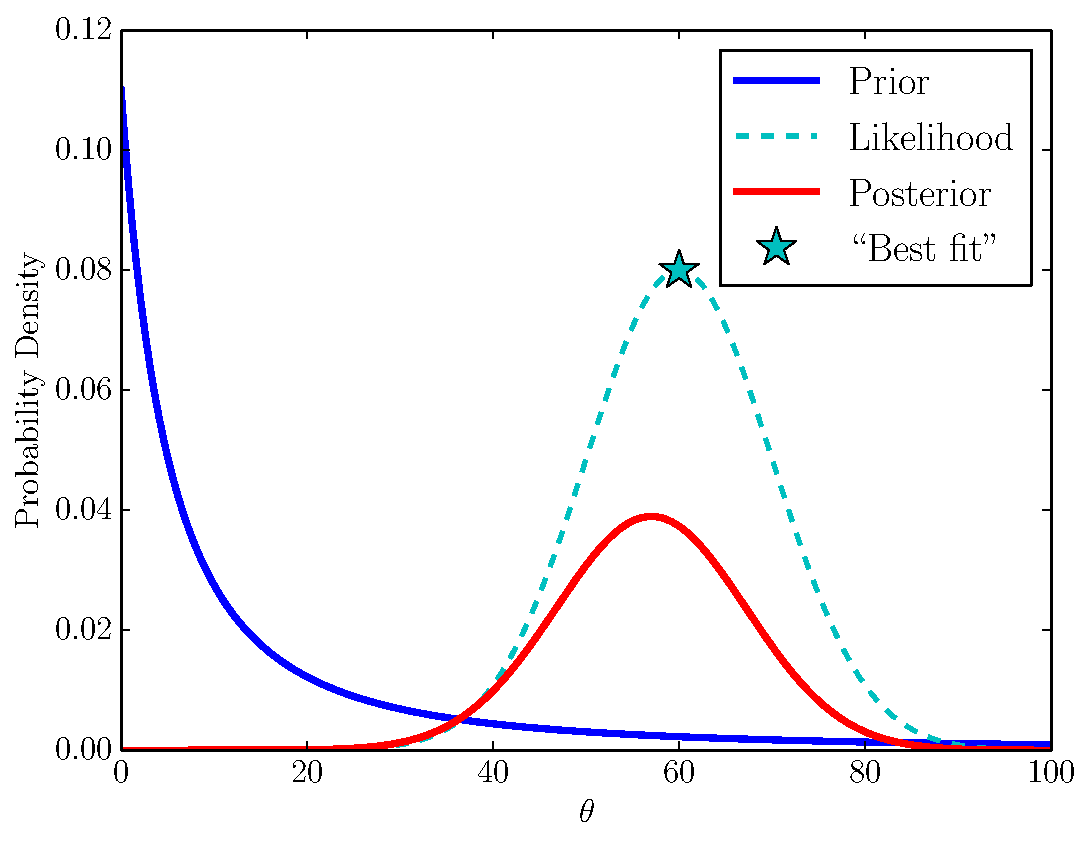
\includegraphics[scale=0.35]{bayes.pdf}
\end{center}
\end{frame}




\begin{frame}[t]{Updating Probabilities: Example}
\begin{center}
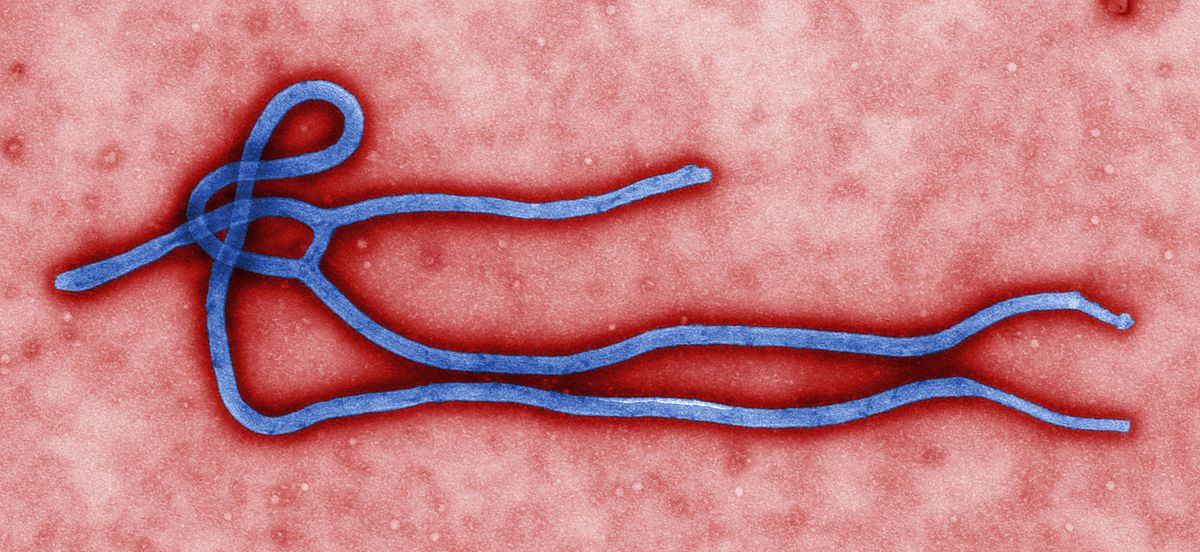
\includegraphics[scale=0.5]{ebola.jpg}
\end{center}
A patient goes to the doctor because he as a fever. Define
\begin{center}
\begin{tabular}{ll}
$H \equiv $ & ``The patient has Ebola''\\
$\bar{H} \equiv $ & ``The patient does not have Ebola''.
\end{tabular}
\end{center}

\end{frame}

\begin{frame}[t]{Updating Probabilities: Example}
Based on all of her knowledge, the doctor assigns probabilities to the two
hypotheses.
\begin{eqnarray*}
P(H) &=& 0.01\\
P(\bar{H}) &=& 0.99
\end{eqnarray*}

But she wants to test the patient to make sure.
\end{frame}



\begin{frame}[t]{Updating Probabilities: Example}
The patient is tested. Define

\begin{center}
\begin{tabular}{ll}
$D \equiv $ & ``The {\bf test says} the patient has Ebola''\\
$\bar{D} \equiv $ & ``The {\bf test says} the patient does not have Ebola''.
\end{tabular}
\end{center}

If the test were perfect, we'd have $P(D | H) = 1$, $P(\bar{D} | H) = 0$,
$P(D | \bar{H}) = 0$, and $P(\bar{D} | \bar{H}) = 1$.
\end{frame}


\begin{frame}[t]{Updating Probabilities: Example}
The Ebola test isn't perfect. Suppose there's a 5\% probability it simply gives
the wrong answer. Then we have:

\begin{eqnarray*}
P(D | H)   &=& 0.95\\
P(\bar{D} | H) &=& 0.05\\
P(D | \bar{H})   &=& 0.05\\
P(\bar{D} | \bar{H}) &=& 0.95
\end{eqnarray*}

\end{frame}

\begin{frame}[t]{Updating Probabilities: Example}
Overall, there are four possibilities, considering whether the patient has
Ebola or not, and what the test says.

\begin{center}
$(H, D)$\\
$(\bar{H}, D)$\\
$(H, \bar{D})$\\
$(\bar{H}, \bar{D})$
\end{center}


\end{frame}

\begin{frame}[t]{Updating Probabilities: Example}
The probabilities for these four possibilities can be found using the product
rule.
\begin{eqnarray*}
P(H, D) &=& 0.01 \times 0.95\\
P(\bar{H}, D) &=& 0.99 \times 0.05\\
P(H, \bar{D}) &=& 0.01 \times 0.05\\
P(\bar{H}, \bar{D}) &=& 0.99 \times 0.95\\
\end{eqnarray*}
\vspace{-45pt}

These four possibilities are {\bf mutually exclusive} (only one of them is true)
and exhaustive (it's not ``something else''), so the probabilities add up to 1.

\end{frame}

\begin{frame}[t]{Updating Probabilities: Example}
The test results come back and say that the patient has Ebola. That is, we've
learned that $D$ is true. So we can confidently rule out those possibilities
where $D$ is false:

\begin{eqnarray*}
P(H, D) &=& 0.01 \times 0.95\\
P(\bar{H}, D) &=& 0.99 \times 0.05\\
{\color{red} P(H, \bar{D})} &=& {\color{red} 0.01 \times 0.05}\\
{\color{red} P(\bar{H}, \bar{D})} &=& {\color{red} 0.99 \times 0.95}\\
\end{eqnarray*}


\end{frame}


\begin{frame}[t]{Updating Probabilities: Example}
We are left with these two possibilities.

\begin{eqnarray*}
P(H, D) &=& 0.01 \times 0.95\\
P(\bar{H}, D) &=& 0.99 \times 0.05
\end{eqnarray*}

It would be strange to modify these probabilities just because we deleted the
other two. The only thing we have to do is renormalise them, by dividing by the total, so they sum to 1 again.
\end{frame}

\begin{frame}[t]{Updating Probabilities: Example}
Normalising, we get

\begin{eqnarray*}
P(H | D) &=& (0.01 \times 0.95)/(0.01 \times 0.95 + 0.99\times0.05) = 0.161\\
P(\bar{H} | D) &=& (0.99 \times 0.05)/(0.01 \times 0.95 + 0.99\times0.05) = 0.839
\end{eqnarray*}
\end{frame}

\begin{frame}[t]{Moral}
Bayesian updating is completely equivalent to:
\begin{itemize}
\item Writing a list of possible answers to your question
\item Giving a probability to each
\item Deleting the ones that you discover are false.
\end{itemize}

It just seems more complicated than this because we often apply it to more
complex sets of hypotheses.
\end{frame}



\begin{frame}[t]{Transit Example}
This example is quite simple, yet it is complex enough to demonstrate many
important principles.
\vspace{1cm}

It is also closely related to many astronomical situations!
\end{frame}


\begin{frame}[t]{Transit Example}
\begin{figure}
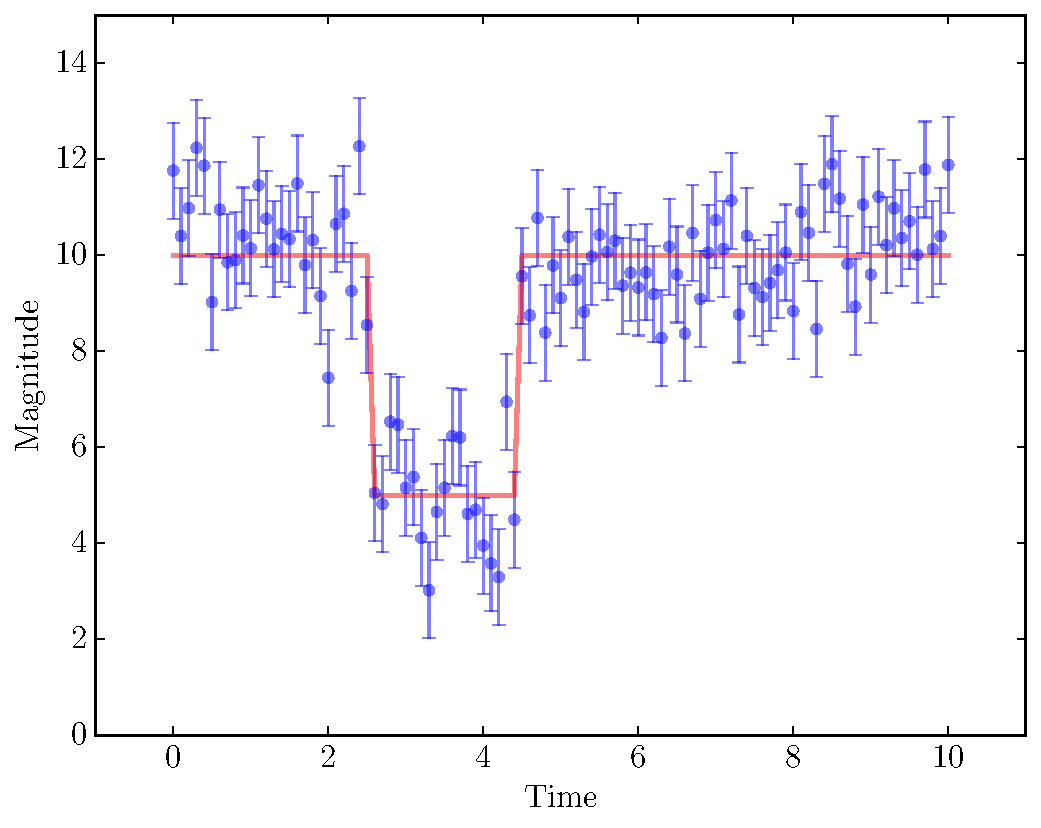
\includegraphics[scale=0.4]{Code/transit_data.pdf}
\end{figure}
\end{frame}



\begin{frame}[t]{Related to the transit example...}
\begin{itemize}
\item Realistic exoplanet transits
\item Finding emission/absorption lines in spectra
\item Finding stars/galaxies in an image
\item ¡Y mucho más!
\end{itemize}
\end{frame}


\begin{frame}[t]{Transit Example: The Truth}
The red curve was:
\begin{eqnarray*}
\mu(t) &=& \left\{
\begin{array}{lr}
10, & 2.5 \leq t \leq 4.5\\
5,  & \textnormal{otherwise}.
\end{array}
\right.
\end{eqnarray*}

\begin{figure}
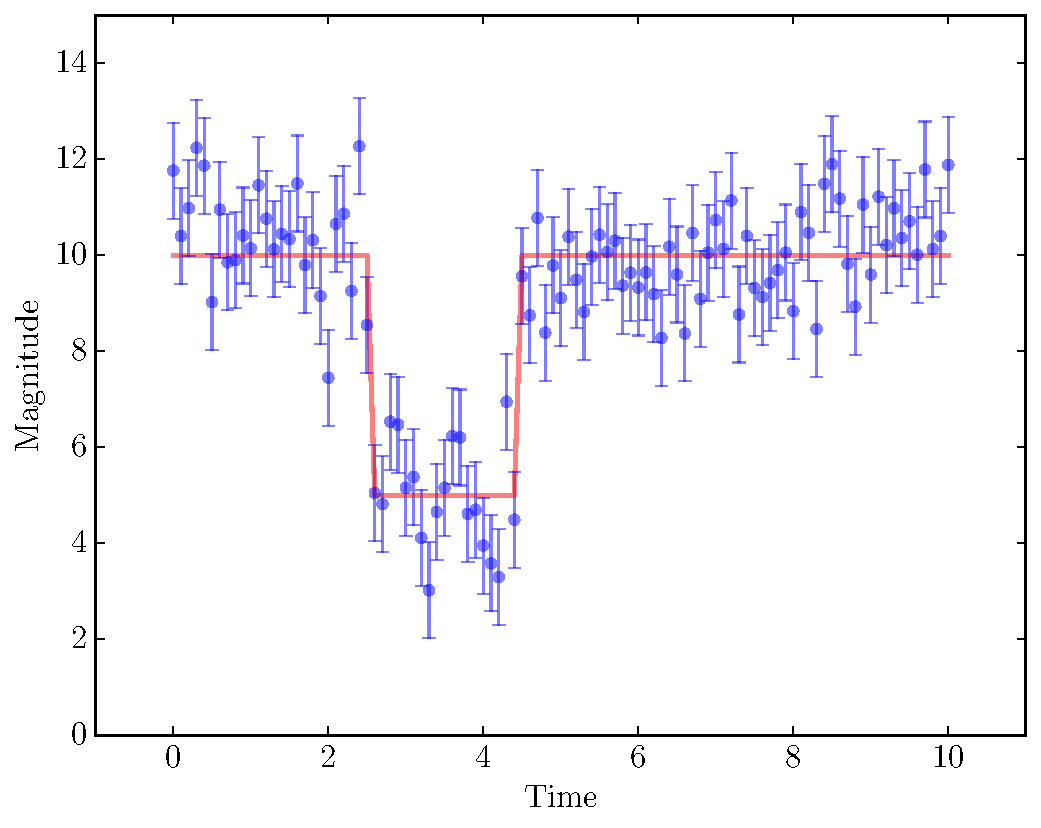
\includegraphics[scale=0.3]{Code/transit_data.pdf}
\end{figure}
\end{frame}

\begin{frame}[fragile, t]{Transit Example: The Truth}
The red curve was:
\begin{eqnarray*}
\mu(t) &=& \left\{
\begin{array}{lr}
10, & 2.5 \leq t \leq 4.5\\
5,  & \textnormal{otherwise}.
\end{array}
\right.
\end{eqnarray*}

and the noise was added like this:
\begin{minted}[mathescape,
               numbersep=5pt,
               gobble=2,
               frame=lines,
               framesep=2mm]{python}
  # Add noise
  sig = 1.
  y += sig*rng.randn(y.size)
\end{minted}
\end{frame}

\begin{frame}[fragile, t]{Transit Example: Inference}
Let's fit the data with this model:
\begin{eqnarray*}
\mu(t) &=& \left\{
\begin{array}{lr}
A, & (t_c - w/2) \leq t \leq (t_c + w/2)\\
A-b,  & \textnormal{otherwise}.
\end{array}
\right.
\end{eqnarray*}

We don't know $A$, $b$, $t_c$, and $w$. But we do know the data $D$.
\end{frame}



\begin{frame}[fragile, t]{Transit Example: Parameters}
We don't know $A$, $b$, $t_c$, and $w$.
These are our unknown parameters. Let's find the posterior.

\begin{eqnarray*}
p(A, b, t_c, w | D) &=& \frac{p(A, b, t_c, w)p(D | A, b, t_c, w)}{p(D)}
\end{eqnarray*}
\end{frame}

\begin{frame}[fragile, t]{Transit Example: Problems I}
The posterior is given by:
\begin{eqnarray*}
p(A, b, t_c, w | D) &=& \frac{p(A, b, t_c, w)p(D | A, b, t_c, w)}{p(D)}
\end{eqnarray*}

But...\\
How do we choose the {\it prior}, $p(A, b, t_c, w)$?\\
How do we choose the {\it likelihood}, $p(D | A, b, t_c, w)$?\\
How do we find $p(D)$?
\end{frame}


\begin{frame}[t]{Choosing priors}
The prior $p(A, b, t_c, w)$
describes what values are plausible, without taking the data into account.

Using the product rule, we can break this down:
\begin{eqnarray*}
p(A, b, t_c, w) &=& p(A) p(b | A) p(t_c | b, A) p(w | t_c, b, A)
\end{eqnarray*}
Often, we can assume the prior factorises like this (i.e. the priors are
{\bf independent}):
\begin{eqnarray*}
p(A, b, t_c, w) &=& p(A) p(b) p(t_c) p(w)
\end{eqnarray*}


\end{frame}


\begin{frame}[t]{Choosing priors}
Often, before we get the data, we have a lot of uncertainty about the
values of the parameters. That's why we wanted the data!

This motivates {\bf vague priors}.

\end{frame}


\begin{frame}[t]{Uniform Priors}
Let's just use wide uniform priors.

e.g.
\begin{eqnarray*}
p(A) = \left\{
\begin{array}{lr}
\frac{1}{200}, & -100 \leq A \leq 100\\
0, & \textnormal{otherwise.}
\end{array}
\right.
\end{eqnarray*}

Abbreviated:
\begin{eqnarray*}
p(A) \sim \textnormal{Uniform}(-100, 100)
\end{eqnarray*}
Or even more concisely:
\begin{eqnarray*}
A \sim U(-100, 100)
\end{eqnarray*}

\end{frame}


\begin{frame}[t]{Uniform Priors}
For all four parameters:

\begin{eqnarray*}
A &\sim& U(-100, 100)\\
b &\sim& U(0, 10)\\
t_c &\sim& U(t_{\rm min}, t_{\rm max})\\
w &\sim& U(0, t_{\rm max} - t_{\rm min})
\end{eqnarray*}

Where $t_{\rm min}$ and $t_{\rm max}$ give the time range of the dataset.
Question: is this legitimate? Are we using the data to set our priors?

\end{frame}


\begin{frame}[t]{Sampling Distribution / Likelihood}
Let's assume ``gaussian noise'':

\begin{eqnarray*}
p(y_i | A, b, t_c, w) &=& \prod_{i=1}^N \frac{1}{\sigma_i\sqrt{2\pi}}
\exp\left[
-\frac{1}{2\sigma_i^2}\left(y_i - m(t_i; A, b, t_c, w)\right)^2
\right].
\end{eqnarray*}
or more concisely:
\begin{eqnarray*}
y_i | A, b, t_c, w \sim \mathcal{N}\left(m(t_i; A, b, t_c, w), \sigma_i^2\right).
\end{eqnarray*}

\end{frame}


\begin{frame}[fragile, t]{Transit Example: Problems II}
Even if we can calculate the posterior $p(A, b, t_c, w | D)$, it is still a
probability distribution over a four-dimensional space.\\
\vspace{20pt}
{\bf How can we understand and visualise it?}
\end{frame}




\begin{frame}[t]{Answer to Problem II: Monte Carlo}
\begin{columns}[T]
\begin{column}{0.35\textwidth}
  \vspace{20pt}
  \begin{itemize}
  \setlength{\itemsep}{10pt}
  \item {\bf Marginalisation} becomes trivial
  \item We can quantify all uncertainties we might be interested in
  \end{itemize}
\end{column}
\hfill
\begin{column}{0.5\textwidth}
  \hspace{-30pt}
  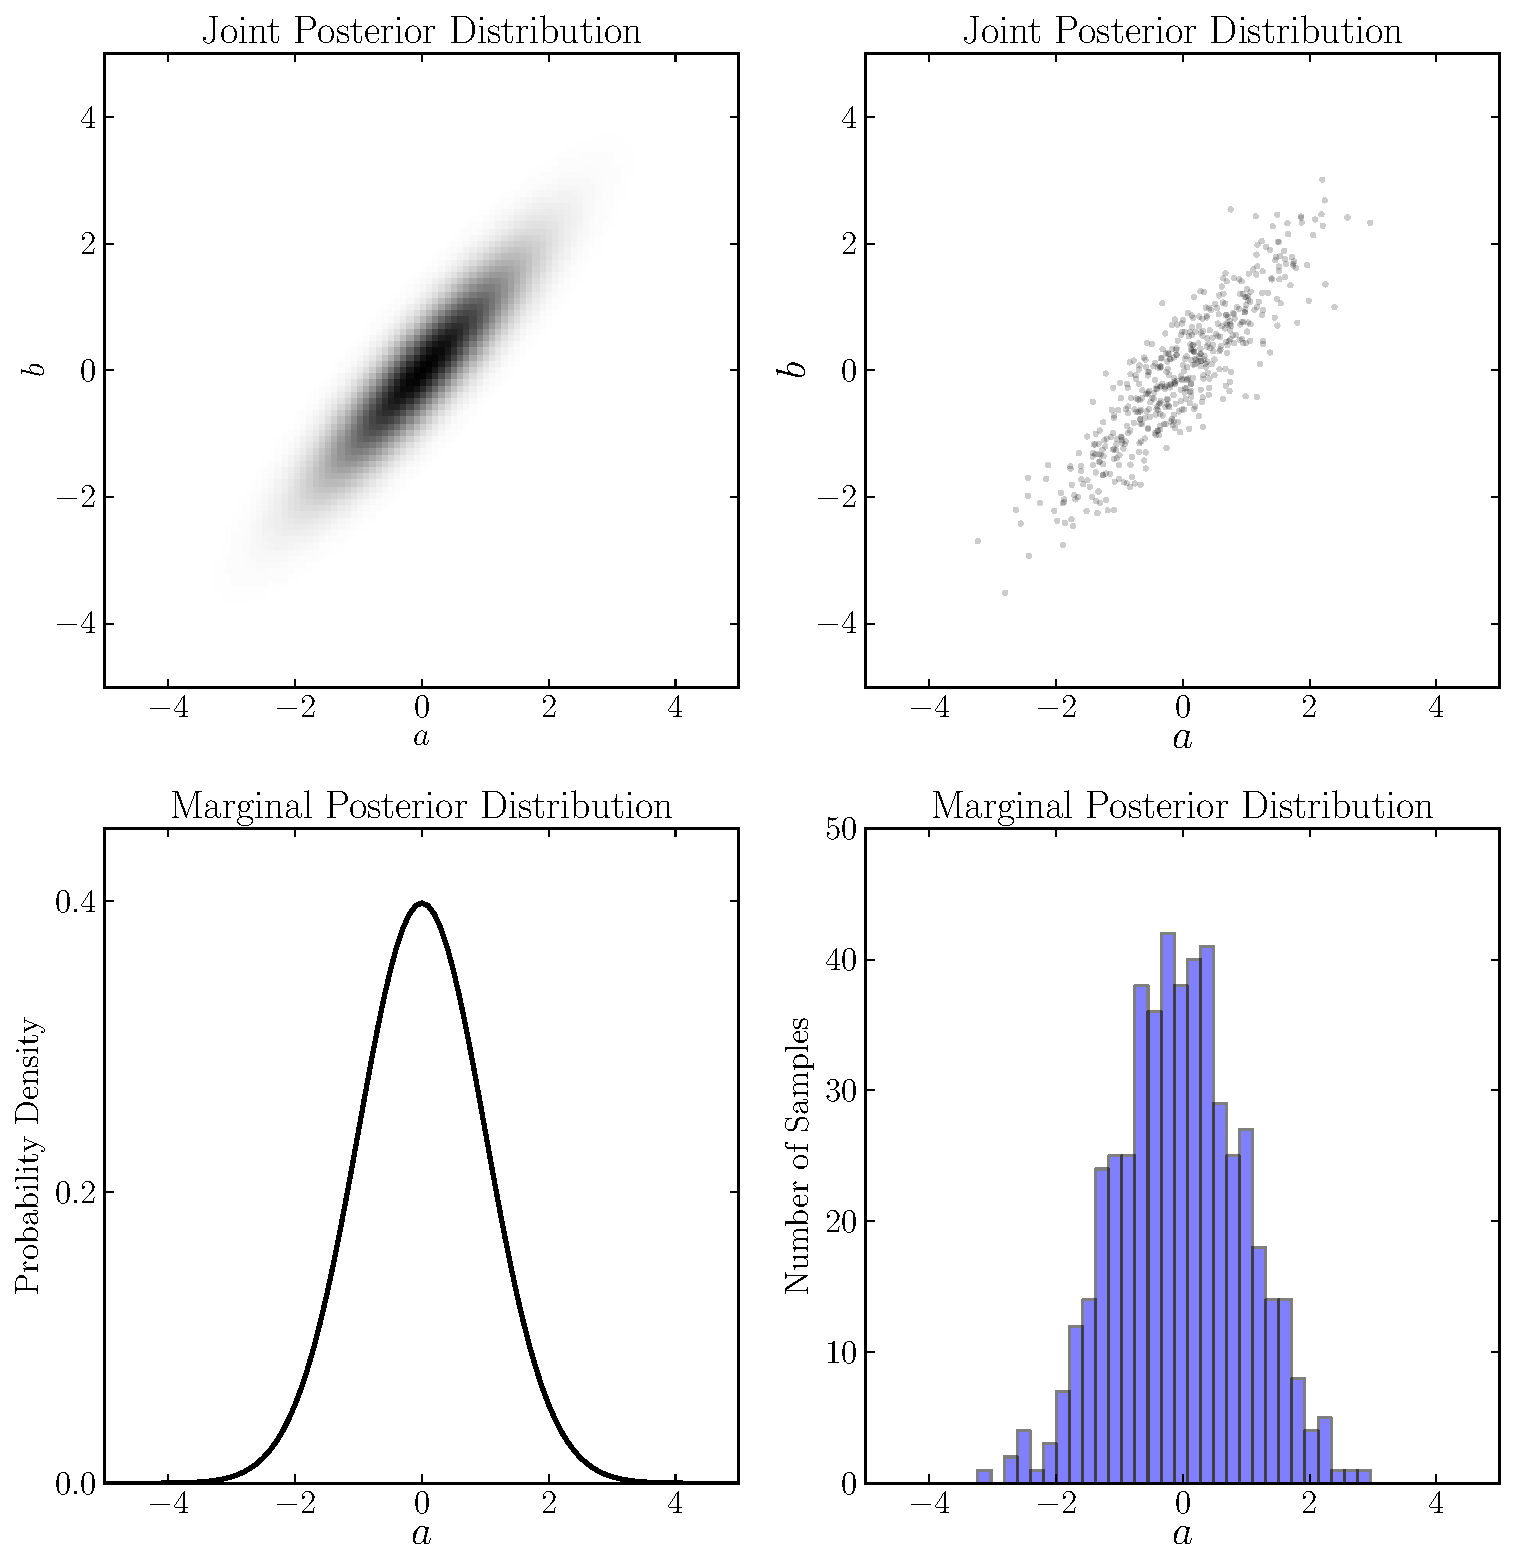
\includegraphics[scale=0.22]{marginalisation.pdf}
\end{column}

\end{columns}
\end{frame}



\begin{frame}[t]{Answer to Problem II: Monte Carlo}
e.g. Posterior mean of $w$:
\begin{eqnarray}
\int w p(A, b, t_c, w | D) \, dA \, db \, dt_c \, dw
\approx \frac{1}{N}\sum_{i=1}^N w_i
\end{eqnarray}
(i.e. just the arithmetic mean). Probability of being in some region $R$:
\begin{eqnarray}
\int_R p(A, b, t_c, w | D) \, dA \, db \, dt_c \, dw
\approx \frac{1}{N}\sum_{i=1}^N \mathds{1}\left(\theta_i \in R \right)
\end{eqnarray}
(i.e. just the fraction of the samples in $R$).
\end{frame}


\begin{frame}[t]{Monte Carlo}
Samples from the posterior are very useful, but how do we generate them?

\begin{center}
Answer: {\bf Markov Chain Monte Carlo}
\end{center}

This is not the {\it only} answer, but it's the most popular.
\end{frame}

\begin{frame}[t]{Monte Carlo}
Samples from the posterior are very useful, but how do we generate them?

\begin{center}
{\tt https://www.youtube.com/watch?v=Vv3f0QNWvWQ}
\end{center}

\end{frame}




\begin{frame}[t]{The Metropolis Algorithm}

\begin{itemize}
\item Start at some point $\theta$ in the hypothesis space.
\item Loop\\
$\{$
  \begin{itemize}
  \item Generate {\bf proposal} from some distribution $q(\theta' | \theta)$
  (e.g. slightly perturb the current position).
  \item With probability $\alpha = \min\left(1, \frac{p(\theta')p(D|\theta')}{p(\theta)p(D|\theta)}\right)$, accept the proposal (i.e. replace $\theta$ with $\theta'$).
  \item Otherwise, stay in the same place.
  \end{itemize}
$\}$
\end{itemize}
\end{frame}

\begin{frame}[t]{Acceptance Probability}
The full acceptance probability is

\begin{eqnarray}
\alpha =
\min\left(1, \frac{q(\theta|\theta')}{q(\theta'|\theta)}\frac{p(\theta')}{p(\theta)}\frac{p(D|\theta')}{p(D|\theta)}\right)
\end{eqnarray}
We'll usually make choices where the $q$s cancel out, and sometimes we'll
choose the $q$s to also cancel out the prior ratio (easier than it sounds).
\end{frame}



\begin{frame}[t]{Implementing the Metropolis Algorithm}
To use Metropolis on the Transit Problem, we'll need functions to:
\begin{itemize}
\item Generate a starting point (I like to draw the parameters from the prior)
\item Make proposals
\item Evaluate the prior distribution at any point
\item Evaluate the likelihood at any point
\end{itemize}
\end{frame}

\begin{frame}[t]{}
Coding...

Note the use of logarithms to avoid overflow and underflow.
\end{frame}


\begin{frame}[t, fragile]{Random Walk Proposals}
\begin{minted}[mathescape,
               numbersep=5pt,
               gobble=2,
               frame=lines,
               framesep=2mm]{python}
  # Generate a proposal
  L = 1.
  proposal = x + L*rng.randn()
\end{minted}

Problem: Efficiency depends strongly on {\tt L}. The only way to know the
optimal value of {\tt L} is to have already solved the problem! Oh dear.
\end{frame}

\begin{frame}[t, fragile]{Heavy-Tailed Random Walk Proposals}
\begin{minted}[mathescape,
               numbersep=5pt,
               gobble=2,
               frame=lines,
               framesep=2mm]{python}
  # Generate a proposal
  L = jump_size*10.**(1.5 - 6.*rng.rand())
  proposal = x + L*rng.randn()
\end{minted}
where {\tt jump\_size} $\approx$ prior width.
Don't need steps much bigger than the prior width, may need them to be much
smaller.
\end{frame}


\begin{frame}[t]{Acceptance Probability}
The full acceptance probability is

\begin{eqnarray}
\alpha =
\min\left(1, \frac{q(\theta|\theta')}{q(\theta'|\theta)}\frac{p(\theta')}{p(\theta)}\frac{p(D|\theta')}{p(D|\theta)}\right)
\end{eqnarray}

For the random walk proposal, the $q$ ratio is equal to 1. Do you understand
why?
\end{frame}

\begin{frame}[t, fragile]{Proposing one parameter at a time}
\begin{minted}[mathescape,
               numbersep=5pt,
               gobble=2,
               frame=lines,
               framesep=2mm]{python}
  def proposal(params):
    new = copy.deepcopy(params)

    which = rng.randint(num_params) # Parameter to change
    L = jump_sizes[which]*10.**(1.5 - 6.*rng.rand())
    new[which] += L*rng.randn()
    return new
\end{minted}
\end{frame}



\begin{frame}[t, fragile]{Useful Plots: The Trace Plot}
\begin{minted}[mathescape,
               numbersep=5pt,
               gobble=2,
               frame=lines,
               framesep=2mm]{python}
  # Trace plot of the first parameter
  plt.plot(keep[:,0])
\end{minted}
\end{frame}

\begin{frame}[t]{Useful Plots: The Trace Plot}
\begin{center}
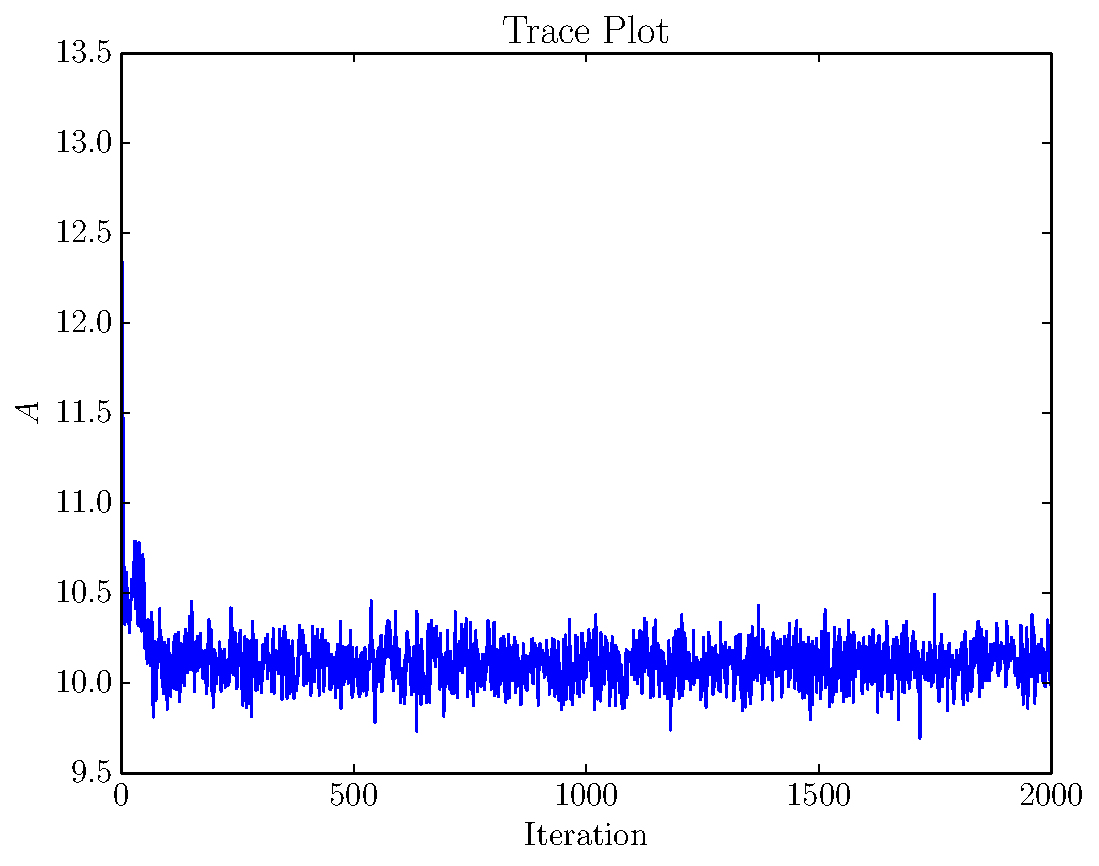
\includegraphics[scale=0.4]{Code/trace_plot.pdf}
\end{center}
\end{frame}


\begin{frame}[t, fragile]{Useful Plots: Marginal Posterior}
\begin{minted}[mathescape,
               numbersep=5pt,
               gobble=2,
               frame=lines,
               framesep=2mm]{python}
  # Marginal posterior for first parameter
  # Excluding first 2000 points
  plt.hist(keep[:,0], 100)
\end{minted}
\end{frame}

\begin{frame}[t]{Useful Plots: Marginal Posterior}
\begin{center}
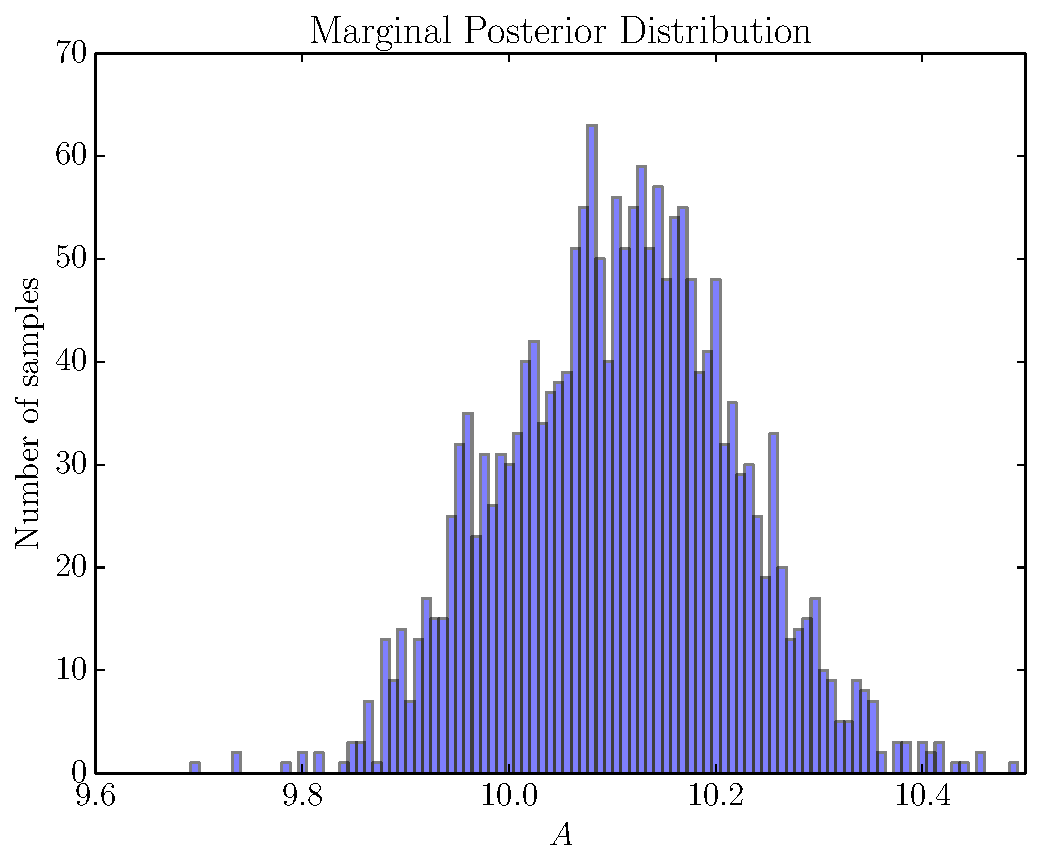
\includegraphics[scale=0.4]{Code/marginal_posterior.pdf}
\end{center}
\end{frame}

\begin{frame}[t]{Comment on Histograms}
If your histograms have so many points that they look perfectly smooth, you
are working on an {\bf easy problem}!
\end{frame}


\begin{frame}[t, fragile]{Useful Plots: Joint Posterior}
\begin{minted}[mathescape,
               numbersep=5pt,
               gobble=2,
               frame=lines,
               framesep=2mm]{python}
  # Joint posterior for first two parameters
  # excluding first 2000 points
  plt.plot(keep[:,0], keep[:,1], 'b.')
\end{minted}
\end{frame}

\begin{frame}[t]{Useful Plots: Joint Posterior}
\begin{center}
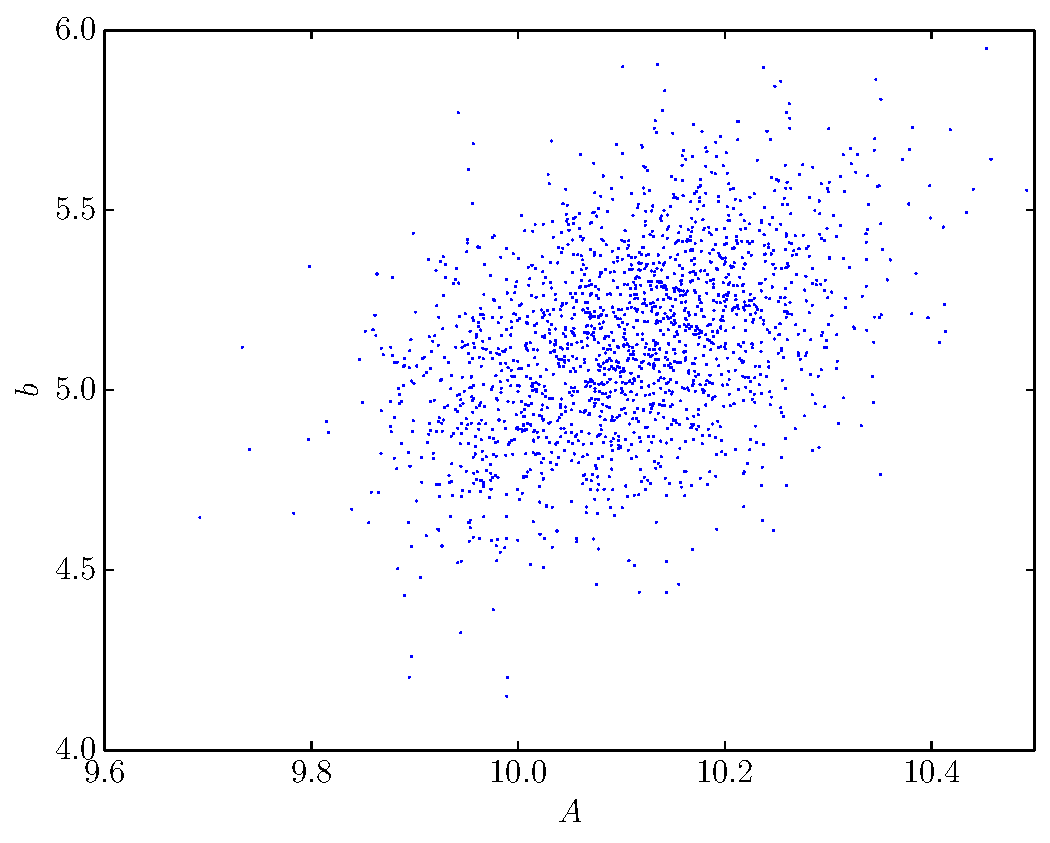
\includegraphics[scale=0.4]{Code/joint_posterior.pdf}
\end{center}
\end{frame}


\begin{frame}[t]{Useful Plots: ``Corner'' or ``Triangle'' Plots}
I like the package {\tt triangle.py} by Dan Foreman-Mackey
({\tt https://github.com/dfm/triangle.py})
\begin{center}
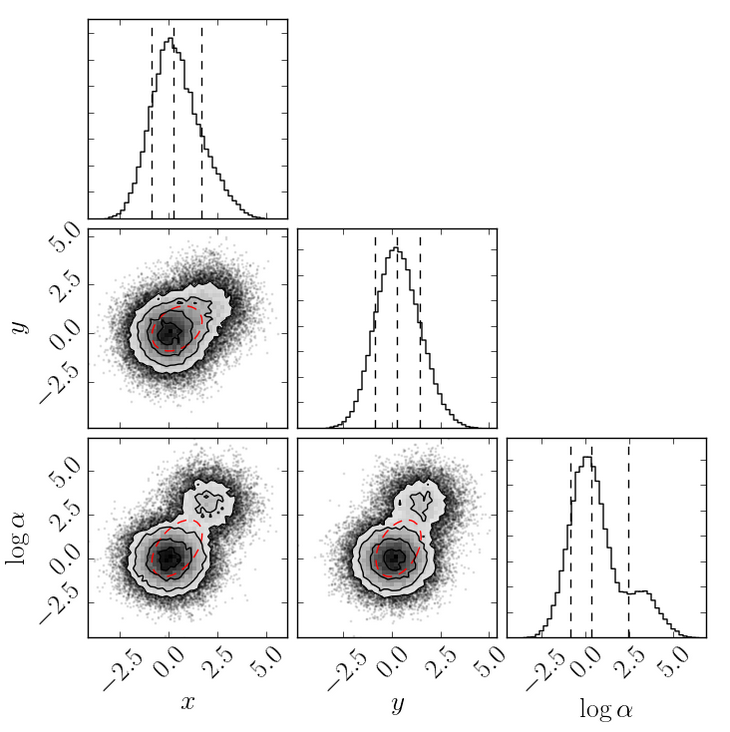
\includegraphics[scale=0.2]{triangle.png}
\end{center}
\end{frame}


\begin{frame}[t]{Useful Summaries}
Posterior distributions can be complicated. Often, we want a simple statement
of the uncertainty. This leads to:

\begin{itemize}
\item Point estimates
\item Credible intervals
\end{itemize}
\end{frame}


\begin{frame}[t, fragile]{Calculating Summaries}
\begin{minted}[mathescape,
               numbersep=5pt,
               gobble=2,
               frame=none,
               framesep=2mm]{python}
  # Posterior mean and sd
  np.mean(keep[:,0])
  np.std(keep[:,0])

  # For median and credible interval
  x = np.sort(keep[:,0].copy())
  # Credible interval (68%)
  x[0.16*len(x)]
  x[0.84*len(x)]
\end{minted}
\end{frame}

\begin{frame}[t]{Bayes' Rule}
Here is Bayes' rule again, with the background information (or assumptions)
made explicit:

\begin{eqnarray*}
p(\theta | D, I) &=& \frac{p(\theta | I)p(D | \theta, I)}{p(D | I)}
\end{eqnarray*}

In any particular application, we make a definite choice of the prior and
the sampling distribution, as well as what $\theta$, $D$, and $I$ are.

\end{frame}


\begin{frame}[t]{What is a parameter?}
What is a parameter?

\begin{itemize}
\item A quantity whose value you would like to know; or
\item A quantity you think you need in order to write down
$p(D | \theta)$.
\end{itemize}

The latter are often called {\bf nuisance parameters}.
For example, in the transit problem we might be interested only in $w$, but
we can't use our ``gaussian noise'' assumption without also including $A$, $b$,
and $t_c$.
\end{frame}




\begin{frame}[t]{In the Transit Example}
Our parameters were:

\begin{eqnarray*}
\theta \equiv \{A, b, t_c, w\}
\end{eqnarray*}

What was our data $D$? We had a data file with three columns: times $\{t_i\}$,
measurements $\{y_i\}$, and ``error bars'' $\{\sigma_i\}$. Was this all our
data $D$?

\end{frame}

\begin{frame}[t]{Answer: No!}
Only the $\{y_i\}$ from the data file was our data. Why? We wrote down
$p(\{y_i\} | \theta, I)$, but we did not write down $p(\{t_i\} | \theta, I)$, or
$p(\{\sigma_i\} | \theta, I)$.

Therefore:

\begin{eqnarray*}
\theta &\equiv& \{A, b, t_c, w\}\\
D &\equiv& \{y_i\}\\
I &\equiv& \{\{t_i\}, \{\sigma_i\}, \textnormal{etc.}\}
\end{eqnarray*}

\end{frame}

\begin{frame}[t]{Assigning Priors}
When assigning our priors (and sampling distribution), it is {\bf completely
legitimate} to use two out of the three columns of our ``data'' file!
\end{frame}

\begin{frame}[t]{Alternative Vague Priors}
How long is a piece of string?
\begin{center}
\includegraphics[scale=0.4]{string.jpg}
\end{center}
\end{frame}

\begin{frame}[t]{Alternative Vague Priors}
How long is a piece of string?

{\bf Twice the distance from the middle to the end.}
\end{frame}

\begin{frame}[t]{Alternative Vague Priors}
Same prior for $\theta$ as for $2\theta \implies$:

\begin{eqnarray*}
p(\theta) \propto \frac{1}{\theta}
\end{eqnarray*}
or
\begin{eqnarray*}
\log(\theta) \sim Uniform(,).
\end{eqnarray*}

By analogy with the log-normal distribution, I like to call this the
{\it log-uniform} distribution.
\end{frame}

\begin{frame}[t]{Why use the log-uniform prior?}
Let $\theta =$ the mass of a galaxy, in solar masses.

``Prior ignorance'' might motivate this prior:

\begin{eqnarray*}
\theta \sim U(0, 10^{15}).
\end{eqnarray*}

\end{frame}

\begin{frame}[t]{Why use the log-uniform prior?}
``Prior ignorance'' might motivate this prior:

\begin{eqnarray*}
\theta \sim U(0, 10^{15}).
\end{eqnarray*}

But this implies:
\begin{eqnarray*}
P(\theta \geq 10^{14}) &=& 0.9\\
P(\theta \geq 10^{12}) &=& 0.999.
\end{eqnarray*}

i.e. we are not ignorant at all, with respect to some questions!

\end{frame}

\begin{frame}[t]{Why use the log-uniform prior?}
\begin{eqnarray*}
\log_{10}(\theta) \sim U(5, 15).
\end{eqnarray*}
implies:
\begin{eqnarray*}
P(\theta \geq 10^{14}) &=& 0.1\\
P(\theta \geq 10^{12}) &=& 0.3
\end{eqnarray*}
or
\begin{eqnarray*}
P(\theta \in [10^{10}, 10^{11}]) = P(\theta \in [10^{11}, 10^{12}])
= P(\theta \in [10^{12}, 10^{13}]) ...
\end{eqnarray*}
\end{frame}

\begin{frame}[t]{Using the log-uniform prior in Metropolis}
Easiest way: just make $\theta' = \log(\theta)$ the parameter:

\begin{itemize}
\item Define proposals, etc, in terms of $\theta'$, which has a uniform prior
\item Just exponentiate it ($\theta = e^{\theta'}$) before using it in the likelihood.
\end{itemize}

Let's apply this to the $w$ (width) parameter in the transit model.
\end{frame}

\begin{frame}[t]{Using the log-uniform prior in Metropolis}
Coding...
\end{frame}

\begin{frame}[t]{Safety Features}
In ``(data) = (model) + noise'' type models, be sceptical of the gaussian
noise assumption. For example, with $N=1000$ data points and $\sigma_i=1$ for
all $i$, one consequence of the sampling distribution (really a prior) is:

\begin{eqnarray}
P\left(\frac{1}{N}\sum_{i=1}^N (y_i - m(t_i; \theta)) \in [-0.06, 0.06]\right)
\approx 95\% 
\end{eqnarray}

Really? Seems a bit confident.
\end{frame}

\begin{frame}[t]{Safety Features}
There are many ways to do this kind of thing. This is just my favourite.
Replace:

\begin{eqnarray*}
y_i | A, b, t_c, w \sim \mathcal{N}\left(m(t_i; A, b, t_c, w), \sigma_i^2\right)
\end{eqnarray*}
with
\begin{eqnarray*}
y_i | A, b, t_c, w \sim \textnormal{Student-}t\left(m(t_i; A, b, t_c, w), (K\sigma_i)^2, \nu\right).
\end{eqnarray*}

\end{frame}

\begin{frame}[t]{$t$ Distributions from Wikipedia}
\begin{center}
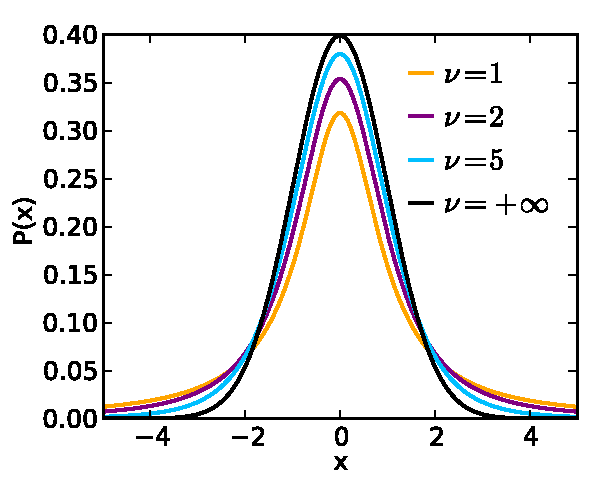
\includegraphics[scale=0.7]{t.pdf}
\end{center}
\end{frame}

\begin{frame}[t]{$t$ Density}
For a single variable...
\begin{eqnarray*}
p(x|\nu, \mu, \sigma) = \frac{\Gamma\left(\frac{\nu + 1}{2}\right)}
{\Gamma\left(\frac{\nu}{2}\right)\sigma\sqrt{\pi\nu}}
\left[1 + \frac{1}{\nu}\frac{(x - \mu)^2}{\sigma^2}
\right]^{-\frac{\nu + 1}{2}}
\end{eqnarray*}

Our likelihood is a product of $N$ terms like this, and we have to code up the log
of the likelihood. Also, remember we're scaling the widths $\sigma$ by a factor $K$.

\end{frame}

